\myparagraph{
    \begin{tcolorbox}[colback=blue!5!white, colframe=blue!75!black]
        Il pattern fornisce un'interfaccia unificata ai servizi forniti di un certo sottosistema.
        La Facade delega le richieste provenienti dai client verso gli oggetti del sottosistema che nasconde. 
        Il suo intento è quello di rendere più semplice l'uso di un sottosistema.
    \end{tcolorbox}

    \vspace{0.1cm}
    \begin{center}
        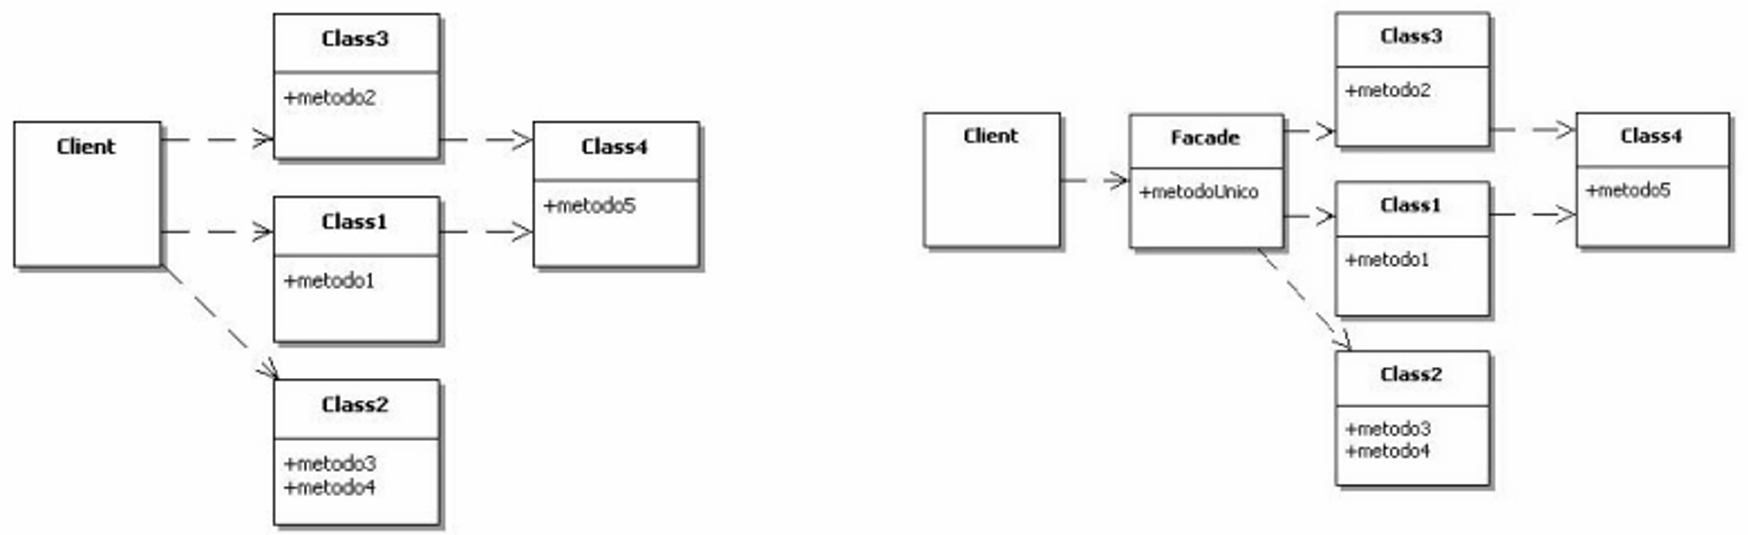
\includegraphics[scale=0.25]{Esercitazione - Design Patterns/Facade.png}
    \end{center}
    I partecipanti del pattern sono:
    \begin{enumerate}
        \item \textbf{Facade}: Conosce le classi responsabili per una richiesta e delega le richieste dei client
        agli oggetti appropriati del sottosistema.
        \item \textbf{Classi del sottosistema}: Implementano le funzionalità del sottosistema e gestiscono il lavoro
        assegnato dal Facade, questo però senza aver alcun riferimento di quest'ultima.
    \end{enumerate}

    Bisogna fare alcune considerazioni riguardo questo pattern:
    \begin{enumerate}
        \item Diminuisce l'accoppiamento tra client e sottosistema.
        \item Nasconde al client le componenti del sottosistema.
        \item Il client può comunque usare direttamente le classi del sottosistema.
    \end{enumerate}
    Si può anche rendere il Facade una classe astratta con sottoclassi concrete per diminuire ulteriormente
    l'accoppiamento. I client possono comunicare con il sottosistema mediante l'interfaccia della classe astratta Facade.

    \mysubsubsectionformatted{Facade vs Adapter}
    \begin{enumerate}
        \item Entrambi sono dei wrapper.
        \item Entrambi si basano su un'interfaccia, però:
        \item \begin{enumerate}
            \item Facade lo semplifica.
            \item Adapter lo converte.
        \end{enumerate}
    \end{enumerate}
}